\documentclass[a4paper,12pt,twocolumn,landscape]{article}

\usepackage{superpack2015}

\usepackage[heightrounded]{geometry}	% heightrounded permet d'afficher les footers correctement
\geometry{hmargin=0.5cm,vmargin=1.5cm}

\setlength{\columnseprule}{0.5pt}		% Ligne séparatrice milieu document
\setlength{\columnsep}{50pt}			% Espace de chaque côté de la ligne
\setlength{\headsep}{15pt}
\addtolength{\textheight}{20pt}
%\setlength{\textwidth}{770pt}
%\setlength{\hoffset}{20pt}

\classichf
	% Nom du style
	{sujet-exercices}
	% Hauteur sous header
	% 14.5pt si une ligne (1 \baselineskip)
	% 29.0pt si deux lignes (2 \baselineskip)
	{14.5pt}
	% Head
	{}
	{\textbf{Exercices : Les fonctions}}
	{}
	% Foot
	{}
	{}
	{}

\classichf
	% Nom du style
	{sujet-po}
	% Hauteur sous header
	% 14.5pt si une ligne (1 \baselineskip)
	% 29.0pt si deux lignes (2 \baselineskip)
	{14.5pt}
	% Head
	{}
	{\textbf{Problèmes ouverts}}
	{}
	% Foot
	{}
	{}
	{}

\classichf
	% Nom du style
	{savoirs}
	% Hauteur sous header
	% 14.5pt si une ligne (1 \baselineskip)
	% 29.0pt si deux lignes (2 \baselineskip)
	{14.5pt}
	% Head
	{}
	{\textbf{Savoirs mis en jeu dans la série d'exercices}}
	{}
	% Foot
	{}
	{}
	{}

%\usepackage{showframe}
%\usepackage{layout}

\begin{document}
\pagestyle{sujet-exercices}	%\thispagestyle{premierepage} pour isoler des styles de pages


\exercice Reprenons la fonction $h$ évoquée dans l'activité
\vspace*{-1em}
\begin{center}
\begin{tikzpicture}[scale=0.5,yscale=3,every node/.style={scale=0.8}]
\tkzInit[xmax=24,xstep=1,ymax=3,ystep=1]
\tkzGrid[sub,
		subxstep=0.25,
		color=gray]
\tkzLabelX
\tkzDrawX[label={\textit{heure le 28/10/2015}},above left=18pt,fill=white]
\tkzLabelY
\tkzDrawY[label={\textit{hauteur d'eau du Gardon d'Al\`es}},below right=8pt]
\draw plot[smooth] file {ales.table.suite};
\tkzAxeX[label=$t$,right=10pt]
\tkzAxeY[label=$h(t)$]
\tkzText(11.8,2.2){$\mathcal{C}_{h}$}
\end{tikzpicture}
\end{center}

\begin{enumerate}
	\item Résoudre graphiquement $h(t) > 2$.
	\item Déterminer graphiquement les antécédents de $2$ par $h$.
	\item Déterminer graphiquement $h(22)$.
	\item Déterminer graphiquement le maximum de la fonction $h$ et la valeur de $t$ pour laquelle on l'obtient.
	\item Déterminer graphiquement les valeurs de~$t$ pour lesquelles la fonction~$h$ est croissante et celles où la fonction~$h$ est décroissante.
	\item Exprimer les réponses de la question précédente sous forme d'intervalles de valeurs de $t$.
	\item Pour chacune des questions précédentes, exprimer en langage courant ce qui est demandé.
	\item Répondre maintenant aux questions de 1. à \addtocounter{enumi}{-2}\theenumi \addtocounter{enumi}{2}.
\end{enumerate}
\input{fonctions1-td-exercice2}
\input{fonctions1-td-exercice3a7}
\newpage
\exercice~\\

\begin{minipage}{0.5\linewidth}
	\definecolor{xdxdff}{rgb}{0.49,0.49,1}
\definecolor{cqcqcq}{rgb}{0.75,0.75,0.75}
\begin{tikzpicture}[line cap=round,line join=round,>=triangle 45,x=1.0cm,y=1.0cm,scale=0.75,xscale=2.45,yscale=0.9,scale=1,every node/.style={scale=0.9}]
\draw [color=cqcqcq,dash pattern=on 2pt off 2pt, xstep=1cm,ystep=3.0cm] (-0.27,-4.53) grid (3.21,6.6);
\draw[->,color=black] (-0.27,0) -- (3.21,0);
\foreach \x in {,0.5,1,1.5,2,2.5,3}
\draw[shift={(\x,0)},color=black] (0pt,2pt) -- (0pt,-2pt) node[below] {\footnotesize $\x$};
\draw[->,color=black] (0,-4.53) -- (0,6.6);
\foreach \y in {-4,-3,-2,-1,1,2,3,4,5,6}
\draw[shift={(0,\y)},color=black] (2pt,0pt) -- (-2pt,0pt) node[left] {\footnotesize $\y$};
\draw[color=black] (0pt,-10pt) node[right] {\footnotesize $0$};
\clip(-0.27,-4.53) rectangle (3.21,6.6);
\draw[smooth,samples=100,domain=-0.27358351729212455:3.2128525876870215] plot(\x,{4*(\x)^2-12*(\x)+5});
\draw [domain=-0.27:3.21] plot(\x,{(--10-8*\x)/2});
\draw (0.67,3) node[anchor=north west] {$g$};
\draw (2.5,2.83) node[anchor=north west] {$f$};
\begin{scriptsize}
\fill [color=xdxdff] (2,-3) circle (1.5pt);
\draw[color=xdxdff] (2.15,-2.79) node {$B$};
\fill [color=xdxdff] (0,5) circle (1.5pt);
\draw[color=xdxdff] (0.09,5.24) node {$A$};
\end{scriptsize}\end{tikzpicture}
\end{minipage}
\begin{minipage}{0.5\linewidth}
Résoudre
\begin{enumerate}
	\item $f(x) = 0$
	\item $f(x) \leqslant 0$\\
	\item $f(x) = 5$
	\item $f(x) \leqslant 5$\\
	\item $f(x) = g(x)$
	\item $f(x) \leqslant g(x)$\\
	\item $0 \leqslant f(x) \leqslant 5$
	\item $-3 \leqslant f(x) \leqslant 0$
\end{enumerate}
\end{minipage}
\exercice~\\

\noindent 
\begin{minipage}{0.50\linewidth}
	\begin{tikzpicture}[scale=0.5,xscale=1,every node/.style={scale=0.75}]
\tkzSetUpPoint[shape=cross]%,size=20pt,color=teal,fill=teal]
\tkzInit[xmin=-0.3,xmax=12.3, ymin=-4.3,ymax=5.3]
\tkzGrid[sub,subxstep=1,subystep=1]
\tkzAxeXY
\tkzFct[smooth,samples=20,domain = -0.3:12.3]{0.05833*(\x)**3-1.05*(\x)**2+4.86667*(\x)-4}
\tkzFct[samples=2,domain = -0.3:12.3]{(-48+8*\x)/12}
\tkzDefPointByFct[draw,ref=A](0)
\tkzLabelPoint[right](A){$A$}
\tkzCrossPoint{A}
\tkzDefPointByFct[draw,ref=B](6)
\tkzLabelPoint[above](B){$B$}
\tkzCrossPoint{B}
\tkzDefPointByFct[draw,ref=C](12)
\tkzLabelPoint[above left](C){$C$}
\tkzCrossPoint{C}
\tkzText(8.5,2.5){$\mathcal{C}_{g}$}
\tkzText(1.5,2.5){$\mathcal{C}_{f}$}
\end{tikzpicture}
\end{minipage}
\begin{minipage}{0.50\linewidth}
\begin{enumerate}
	\item Dresser le \underline{tableau de variation} de~$f$ pour \mbox{$x \in [0~;~12]$}.\\
	\item Dresser le \underline{tableau de signes} de~$g$ pour \mbox{$x \in [0~;~12]$}.\\
	\item Entourer la bonne solution sur chaque ligne du tableau.
\end{enumerate}
\end{minipage}

\begin{center}
\begin{tabular}{|c|c|}
\hline 
\rule[-1ex]{0pt}{2.5ex} $f(x) \leqslant g(x)$ pour $x \in [0~;~6]$ & $f(x) \leqslant g(x)$ pour $x \in [6~;~12]$ \\ 
\hline 
\rule[-1ex]{0pt}{2.5ex} $f(x) \geqslant 0$ pour $x \in [1~;~6]$ & $f(x) \geqslant 0$ pour $x \in [6~;~11]$ \\ 
\hline 
\rule[-1ex]{0pt}{2.5ex} $f(x) \ge	qslant 0$ pour $x \in [6~;~11]$ & $f(x) \leqslant 0$ pour $x \in [0~;~1] \cup [6~;~11]$ \\ 
\hline 
\end{tabular} 
\end{center}
\exercice On considère le quadrilatère tournant vu lors d'une activité:\\[1em] \noindent
$ABCD$ représente une feuille au format~$A4$ c'est-à-dire un rectangle de côtés $AB = 29,7cm$ et $BC = 21cm$.\\
On place $M$ sur $[AB]$.\\
On place ensuite $N$ sur $[BC]$, $P$ sur $[CD]$ et $Q$ sur $[DA]$ tels que~:\\ $AM = BN = CP = DQ$\\[1em]
On pose $x$ la longueur $AM$.
\begin{center}
	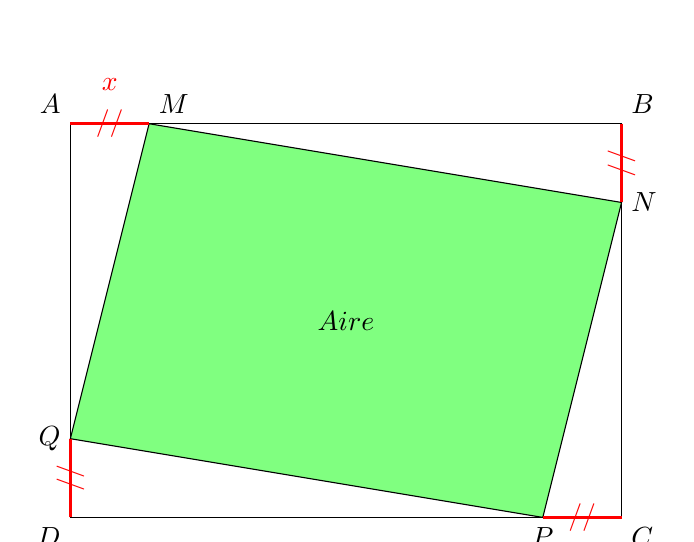
\begin{tikzpicture}[scale=1,every node/.style={scale=1}]
	\coordinate (A) at (0,0);
	\coordinate (B) at (7,0);
	\coordinate (C) at (7,-5);
	\coordinate (D) at (0,-5);
	\coordinate (M) at (1,0);
	\coordinate (N) at (7,-1);
	\coordinate (P) at (6,-5);
	\coordinate (Q) at (0,-4);
	\coordinate (S) at (7/2,-5/2);
	\draw (A) rectangle ++(7,-5);
	\draw (A)--(B)--(C)--(D)--cycle;
%	\draw [very thick,red] (A)--(M) node [midway,above] {$x$};
	\draw [black,fill=green!50] (M)--(N)--(P)--(Q)--cycle;
	\draw (A) node[above left] {$A$};
	\draw (B) node[above right] {$B$};
	\draw (C) node[below right] {$C$};
	\draw (D) node[below left] {$D$};
	\draw (M) node[above right] {$M$};
	\draw (N) node[right] {$N$};
	\draw (P) node[below] {$P$};
	\draw (Q) node[left] {$Q$};
	\draw (S) node {$Aire$};
%	\foreach \point in {A, B, C, D}
%		\draw (\point) node[above left] {$\point$};
	\draw [red,very thick] (A)--(M)node[midway,sloped]{$//$};
	\draw [red,very thick] (B)--(N)node[midway,sloped]{$//$};
	\draw [red,very thick] (C)--(P)node[midway,sloped]{$//$};
	\draw [red,very thick] (D)--(Q)node[midway,sloped]{$//$};
	\draw (0.5,0.5) node [red] {$x$};
\end{tikzpicture}

\end{center}

\begin{enumerate}
	\item Montrez que les triangles $AMQ$ et $CPN$ sont identiques.
	\item De même pour les triangles $BNM$ et $DQP$.
	\item Déterminez l'aire totale de la surface recouverte par les 4 triangles précédents.
	\item Faites une phrase qui décrit le fait que l'aire verte peut s'écrire comme une fonction de $x$ dont on précisera le domaine de définition.
	\item Montrez que cette fonction a pour expression : \[a(x) = 2x^2 - 50,7x + 623,7\]
	\item Déterminez le minimum de cette fonction par le moyen de votre choix : lecture graphique, approximation par différents essais\ldots
\end{enumerate}
\newpage
\exercice Abonnement à la piscine

\vspace*{\stretch{1}}

Anna, Tom et John veulent aller à la piscine cette année. La piscine qu'ils ont choisie propose les tarifs suivants :

\vspace*{\stretch{1}}

\begin{enumerate}[~]
	\item \textbf{Tarif 1} L'entrée à \EUR{3,50}.
	\item \textbf{Tarif 2} Un abonnement de \EUR{50} donnant accès à la salle + \EUR{2} par entrée.
	\item \textbf{Tarif 3} Un abonnement de \EUR{180} pour un accès illimité pendant un an.
\end{enumerate}

\vspace*{\stretch{1}}

Ils ont tous les trois une pratique différente et plus ou moins intense de la natation. On se propose de leur indiquer quel est l'abonnement le plus avantageux pour chacun d'entre eux en fonction de leur fréquentation de la piscine. Tom estime qu'il ira environ 2 fois par mois à la piscine. Anna compte se rendre à la piscine une fois par semaine. Pour maintenir son niveau national, John ira au moins deux fois par semaine.

\vspace*{\stretch{1}}

\begin{enumerate}[1)~~~]
\item Quel est le prix pour 20 entrées dans les trois cas ?

\vspace*{\stretch{1}}

\item Exprimer les fonctions $f_1(x)$, $f_2(x)$ et $f_3(x)$ qui représentent respectivement le prix à payer en fonction de \mbox{$x=$ \og nombre de séances\fg} avec les tarifs 1, 2 et 3.

%\fbox{$f_1(x)=$~~~~~~~~~~~~~~~~~~~~~~~~~~~~~~~~~~~~~~}
%
%\fbox{$f_2(x)=$~~~~~~~~~~~~~~~~~~~~~~~~~~~~~~~~~~~~~~}
%
%\fbox{$f_3(x)=$~~~~~~~~~~~~~~~~~~~~~~~~~~~~~~~~~~~~~~}

\vspace*{\stretch{1}}

\item Reproduire et remplir le tableau suivant avec le prix à payer en fonction du nombre d'entrées pour chaque tarif.
	\begin{center}
		\begin{tabular}{|>{\centering}m{100pt}|>{\centering}m{30pt}|>{\centering}m{30pt}|>{\centering}m{30pt}|>{\centering}m{30pt}|m{30pt}|}
		\hline 
	%			&  &   &   &   & \\
		Nombre d'entrées & $10$ & $20$ & $30$ & $40$ & $~~50$ \\
	%			&  &   &   &   & \\
		\hline
	%			&  &   &   &   &	\\
		Prix 1 	&  &   &   &   &	\\ 
	%			&  &   &   &   &	\\
		\hline 
	%			&  &   &   &   &	\\
		Prix 2 	&  &   &   &   &	\\ 
	%			&  &   &   &   &	\\
		\hline 
	%			&  &   &   &   &	\\
		Prix 3 	&  &   &   &   &	\\ 
	%			&  &   &   &   &	\\
		\hline 
		\end{tabular}~\\~\\
	\end{center}
	
\vspace*{\stretch{1}}

\item Tracer la représentation graphique des fonctions $f_1(x)$, $f_2(x)$ et $f_3(x)$. \textbf{Attention aux unités !} On prendra $2~cm=10$ entrées sur l'axe des abscisses et $1~cm=~$\EUR{20} sur l'axe des ordonnées ou on pourra utiliser le repère fourni par le professeur.	

\vspace*{\stretch{1}}

\item Lire graphiquement~:
		\begin{enumerate}
			\item l'image de 24 par $f_1~$	% : ~~\fbox{$f_1(50)=$~~~~~~~~~~~~~~~~~~}
			\item l'image de 24 par $f_2~$	% : ~~\fbox{$f_2(50)=$~~~~~~~~~~~~~~~~~~}
			\item l'image de 24 par $f_3~$	% : ~~\fbox{$f_3(50)=$~~~~~~~~~~~~~~~~~~}
			\item $\Longrightarrow$ Quel est le tarif le plus intéressant pour 24~entrées ?	% \fbox{Tarif~~~~~}
		\end{enumerate}

\vspace*{\stretch{1}}

\newpage

\item $f_1(x)=70$
		\begin{enumerate}
			\item Mathématiquement, $x$ est l'\textbf{antécédent} de 70.\\ Résoudre graphiquement $f_1(x)=70$.	% : \fbox{\parbox[c][1em][c]{0.15\textwidth}{{$x=$}}}
			\item Que représente concrètement $x$ dans ce cas ?
		\end{enumerate}
		
%\vspace*{\stretch{1}}

\item Résoudre graphiquement $f_1(x)=f_2(x)$.	% : \fbox{\parbox[c][1em][c]{0.15\textwidth}{{$x=$}}}

%\vspace*{\stretch{1}}

\item Déterminer quels tarifs doivent choisir Anna, Tom et John.	% \fbox{Anna : ~~~}~~\fbox{Tom : ~~~}~~\fbox{John : ~~~}

%\vspace*{\stretch{8}}

%\item Retrouver par le calcul le nombre de séances à partir duquel il est plus avantageux de choisir le tarif~2.
%\item Même question pour le tarif 3.
\end{enumerate}

%\begin{center}
%	\begin{tabular}{|>{\centering}m{100pt}|>{\centering}m{30pt}|>{\centering}m{30pt}|>{\centering}m{30pt}|>{\centering}m{30pt}|m{30pt}|}
%	\hline 
%					&  &   &   &   & \\
%	Nombre d'entrées& $10$ & $20$ & $30$ & $40$ & $~~50$ \\
%					&  &   &   &   & \\
%	\hline
%					&  &   &   &   &	\\
%	Prix 1 			& $35$ & $70$ & $105$ & $140$ & $~175$		\\ 
%	$f_1(x)=3,5x$	&  &   &   &   &	\\
%	\hline 
%					&  &   &   &   &	\\
%	Prix 2 			& $70$ & $90$ & $110$ & $130$ & $~150$		\\ 
%	$f_2(x)=2x+50$	&  &   &   &   &	\\
%	\hline 
%					&  &   &   &   &	\\
%	Prix 3		 	& $180$ & $180$ & $180$ & $180$ & $~180$	\\
%	$f_3(x)=180$	&  &   &   &   &	\\ 
%	\hline 
%	\end{tabular}~\\~\\
%\end{center}

%\begin{center}
%	\begin{tabular}{|>{\centering}m{100pt}|>{\centering}m{30pt}|>{\centering}m{30pt}|>{\centering}m{30pt}|>{\centering}m{30pt}|m{30pt}|}
%	\hline 
%%			&  &   &   &   & \\
%	Nombre d'entrées & $10$ & $20$ & $30$ & $40$ & $~~50$ \\
%%			&  &   &   &   & \\
%	\hline
%%			&  &   &   &   &	\\
%	Prix 1 	&  &   &   &   &	\\ 
%%			&  &   &   &   &	\\
%	\hline 
%%			&  &   &   &   &	\\
%	Prix 2 	&  &   &   &   &	\\ 
%%			&  &   &   &   &	\\
%	\hline 
%%			&  &   &   &   &	\\
%	Prix 3 	&  &   &   &   &	\\ 
%%			&  &   &   &   &	\\
%	\hline 
%	\end{tabular}~\\~\\
%\end{center}

%%
%% Graphique
%%
%%
%%\clearpage
%%\begin{rotate}{-90}
%%\begin{tikzpicture}[
%%						xscale=7,
%%						yscale=1.7,
%%						scale=0.04,
%%						every node/.style={scale=1}
%%					]
%%	\coordinate(O) at (0,0);
%%	\draw (O) node [below left] {$O$};
%%	\draw [->,>=stealth, very thick] (-4,0)--(90,0);
%%	\draw [->,>=stealth, very thick] (0,-30)--(0,220);
%%	\draw [dashed,red] (100/3,0)--(100/3,350/3);
%%	\draw (100/3,0) node [below] {$\dfrac{100}{3}$};
%%	\draw [dashed,red] (65,0)--(65,180);
%%	\draw (0,180) node [left] {$180$};
%%	\foreach \nombre in {10, 20, ..., 70, 65}
%%		\draw (\nombre,-5)
%%			node [below] {\nombre}
%%			node [above] {$|$};
%%%	\draw [dashed,red] (0,350/3)--(100/3,350/3);
%%%	\draw (0,350/3) node [left] {$\dfrac{350}{3} \approx 116,66$};
%%%	\draw [->,>=latex,dashed,red] (1,-1)--(1,25);
%%%	\draw [->,>=latex,dashed,red] (1,-1)--(1,12.5);
%%%	\draw [->,>=latex,dashed,red] (1,25)--(0,25);
%%%	\draw (1,-1) node [below] {$x$};
%%%	\draw (-0.1,25) node [left] {$f(x)$};
%%%	\draw [dashed] (5,-1)--(5,25);
%%%	\draw [->,>=stealth, very thick] (0,0)--(1,0);
%%%	\draw [->,>=stealth, very thick] (0,0)--(0,1);
%%	\draw plot [domain=0:60] (\x,{3.5*(\x)}) node [above] {$f_1(x)=3,5x$};
%%	\draw plot [domain=0:70,near end] (\x,{50+(2*\x)}) node [above] {$f_2(x)=2x+50$};
%%	\draw plot [domain=0:80,near end] (\x,{180}) node [below] {$f_3(x)=180$};
%%\end{tikzpicture}~\\~\\
%%\end{rotate}

%\begin{tikzpicture}[xscale=10,scale=0.1,every node/.style={scale=1}]
%	\coordinate(O) at (0,0);
%	\draw (O) node [below left] {$O$};
%	\draw [->,>=stealth, very thick] (-2,0)--(8,0);
%	\draw [->,>=stealth, very thick] (0,-5)--(0,40);
%	\draw [->,>=latex, dashed,red] (-0.1,25)--(1,25);
%	\draw [->,>=latex, dashed,red] (-0.1,25)--(5,25);
%	\draw [->,>=latex, dashed,red] (1,25)--(1,12.5);
%	\draw [->,>=latex, dashed,red] (5,25)--(5,12.5);
%	\draw [->,>=latex, dashed,red] (1,25)--(1,0);
%	\draw [->,>=latex, dashed,red] (5,25)--(5,0);
%	\draw [dashed,red] (1,-1)--(1,25);
%	\draw [dashed,red] (5,-1)--(5,25);
%	\draw (-0.1,25) node [left] {$y$};
%	\draw (1,-1) node [below] {$x_1$};
%	\draw (5,-1) node [below] {$x_2$};
%%	\draw [->,>=stealth, very thick] (0,0)--(1,0);
%%	\draw [->,>=stealth, very thick] (0,0)--(0,1);
%	\draw plot [domain=-1:7] (\x,{2*(\x)^2 - 12*(\x) + 35});
%\end{tikzpicture}
%\hspace*{\stretch{1}}

\exercice On appelle $h$ la fonction représentée graphiquement ci-dessous. Résolvez graphiquement~:\\

\begin{minipage}{0.35\linewidth}
	\begin{enumerate}
		\item $h(x) \leqslant 0$ %\\ \rouge{$\mathbf{x \in \left[ - ~;~ \right]}$}\\
		\item $h(x) \leqslant -5$ %\\ \rouge{$\mathbf{x \in \left[ - ~;~ \right]}$}\\
		\item $-5 \leqslant h(x) \leqslant 0$ %\\ \rouge{$\mathbf{x \in \left[ - ~;~ \right]}$}\\
	\end{enumerate}
\end{minipage}
\begin{minipage}{0.5\linewidth}
	\begin{enumerate}
		\setcounter{enumi}{3}
		\item Tracez la droite $d(x)=-x-6$
		\item Résolvez $h(x) \leqslant d(x)$
		\item[~] ~
	\end{enumerate}
\end{minipage}
\begin{center}
	\begin{tikzpicture}[scale=0.75,xscale=1,every node/.style={scale=0.75}]
%\tkzSetUpPoint[shape=cross,size=20pt,color=teal,fill=teal]
\tkzInit[xmin=-7.5,xmax=8.75,xstep=1, ymin=-6,ymax=2]
\tkzGrid[sub,subxstep=1,subystep=1]
\tkzAxeXY
\tkzFct[smooth,samples=100,domain = -7.5:8.75]{((\x)+6)*((\x)-6)/((\x)+8)}
%\tkzFct[samples=2,domain = -7.5:8.75]{-\x-6}
%\tkzDefPointByFct[draw,ref=A](-6)
%\tkzLabelPoint[above right](A){$A$}
%\tkzCrossPoint{A}
%\tkzDefPointByFct[draw,ref=B](-1)
%\tkzLabelPoint[above left](B){$B$}
%\tkzCrossPoint{B}
%\tkzText(8.5,2.5){$\mathcal{C}_{g}$}
\tkzText(1.7,-2.7){$\mathcal{C}_{f}$}
\end{tikzpicture}
\end{center}

\exerciceprime On s'intéresse à la fonction $h$ représentée ci-dessous

\begin{enumerate}
	\item Peut-on dresser le tableau de signes de cette fonction sur $\mathbb{R}$ à l'aide de la courbe représentative dont on dispose à l'exercice précédent~?
	\item Cette fonction a pour expression $h : x \mapsto \dfrac{(x+6)(x-6)}{x+8}$\\
			Dressez les tableaux de signes de la fonction $h$ pour $x \in [-7,20]$, puis~pour~$x \in \mathbb{R}$.
\end{enumerate}
\newpage
\input{fonctions1-td-exercice13}
\newpage
\exercice On appelle $g$ la fonction représentée ci-dessous.\\ Les propositions suvantes sont-elles vraies ou fausses ?

\begin{enumerate}
	\item Quel que soit $x$ appartenant à $[0,10]$, le nombre $g(x)$ est positif ou nul.\footnote{\textbf{Remarque} Cette proposition pourrait s'écrire comme ceci en langage mathématique~: $\forall x \in [0,10],\quad g(x) \geqslant 0$}
	\item Quel que soit $x$ appartenant à $[0,10]$, $g(x)$ est plus grand que 1.
	\item $g(3) \geqslant 0,04$
	\item $g(2) \geqslant 0,1$
	\item $g(2) \geqslant g(1)$
\end{enumerate}
\begin{center}
	\begin{tikzpicture}[scale=0.9]%,xscale=1,yscale=10,every node/.style={scale=0.75}]
\tkzSetUpPoint[shape=cross]%,size=20pt,color=teal,fill=teal]
\tkzInit[xmin=0,xmax=10, ymin=0,ymax=0.14,xstep=1,ystep=0.02]
\tkzGrid[sub,subxstep=1,subystep=0.01]
\tkzAxeXY
%\tkzFct[smooth,samples=200,domain = 0:10]{exp(- exp(((0 - \x)/(2))))}
% Densité de proba de la loi de Gumbel avec \beta = 3
\tkzFct[smooth,samples=200,domain = 0:10]{\x*exp(- \x)/3}
\tkzDefPointByFct[draw,ref=A](3)
\tkzLabelPoint[above right](A){$A$}
\tkzCrossPoint{A}
\tkzDefPointByFct[draw,ref=B](10)
\tkzLabelPoint[above right](B){$B$}
\tkzCrossPoint{B}
%\tkzDefPointByFct[draw,ref=C](0.27229)
%\tkzLabelPoint[red,above right](C){$C$}
%\tkzCrossPoint{C}
%\tkzFct[red,samples=2,domain = 0:10]{-0.007142*\x + 0.07142}
%\tkzText(8.5,2.5){$\mathcal{C}_{g}$}
%\tkzText(1.5,2.5){$\mathcal{C}_{f}$}
\end{tikzpicture}
\end{center}
Ensuite,
\begin{enumerate}
	\setcounter{enumi}{5}
	\item Tracez la droite $\mathcal{D}$ passant par les points $A$ et $B$, elle coupe la courbe représentative de $g$ en $C$.
	\item On notera $C\left(c,~g\left(c\right)\right)$, déterminez l'intervalle sur lequel la fonction~$g$ est au dessus de la droite~$\mathcal{D}$.
	\item Déterminez l'intervalle (ou la réunion d'intervalles) sur lequel (laquelle) la fonction~$g$ est au dessus de la droite~$\mathcal{D}$.
	\item Déterminez l'expression de la fonction affine $d$ en fonction de $x$ représentée par la droite~$\mathcal{D}$.
\end{enumerate}
\newpage
\exercice Soit $f$ la fonction représentée ci-dessous.\footnote[1]{La fonction $f$ porte le nom de fonction inverse que l'on étudiera plus en détails plus tard}\\ L'expression de $f$ est la suivante, $f : x \mapsto \dfrac{1}{x}$.\\[1em] Soient $A$ et $B$ deux points appartenant à la représentation graphique de $f$ et tels que leurs abscisses soient opposées.

\begin{enumerate}
	\item Émettre une conjecture sur les coordonnées du milieu de $[AB]$.
	\item La démontrer.
\end{enumerate}

\begin{center}
	\begin{tikzpicture}[scale=0.85]%,xscale=1,yscale=10,every node/.style={scale=0.75}]
\tkzSetUpPoint[shape=cross]%,size=20pt,color=teal,fill=teal]
\tkzInit[xmin=-7,xmax=7, ymin=-7,ymax=7,xstep=1,ystep=1]
\tkzGrid[sub,subxstep=1,subystep=5]
\tkzAxeXY
%\tkzFct[smooth,samples=200,domain = 0:10]{1 / \x}
% Densité de proba de la loi de Gumbel avec \beta = 3
\tkzFct[smooth,samples=200,domain = -7:-1/7]{1 / \x}
\tkzFct[smooth,samples=200,domain = 1/7:7]{1 / \x}
\tkzDefPointByFct[draw,ref=A](0.5)
\tkzLabelPoint[above right](A){$A$}
\tkzCrossPoint{A}
\tkzDefPointByFct[draw,ref=B](-0.5)
\tkzLabelPoint[left](B){$B$}
\draw[loosely dashed,red] (A) -- (B);
\tkzCrossPoint{B}
%\tkzDefPointByFct[draw,ref=C](0.27229)
%\tkzLabelPoint[red,above right](C){$C$}
%\tkzCrossPoint{C}
%\tkzFct[red,samples=2,domain = 0:10]{-0.007142*\x + 0.07142}
%\tkzText(8.5,2.5){$\mathcal{C}_{g}$}
%\tkzText(1.5,2.5){$\mathcal{C}_{f}$}
\end{tikzpicture}
\end{center}
\newpage
\pagestyle{sujet-po}
\probleme~\\

Vous travaillez pour le service de R\&D d'une célèbre enseigne, spécialiste des aliments conditionnés en conserve.
Vous êtes en charge de la conception d'une nouvelle boîte de conserve pour conditionner ses petits pois.
Le cahier des charges est le suivant.\\

\noindent Vous devez respecter 3 conditions : \\

\begin{enumerate}
	\item La boîte doit être cylindrique,\\
	\item La boîte doit contenir $1L$,\\
	\item Le matériau de construction de la boîte n'ayant aucun intérêt pour l'achat que veut réaliser le consommateur (il veut juste manger des petits pois !), il vous faut utiliser le moins de matière possible pour réaliser cette boîte.\\
\end{enumerate}

\hfill\AUTRAVAIL
\probleme Je souhaite réaliser une boîte (sans couvercle) de volume maximal avec une feuille $A4$ en suivant les étapes suivantes. Aidez-moi~!

\begin{enumerate}
	\item Prenez une feuille $A4$
	\item Ôtez les coins
	\item Pliez selon les pointillés
\end{enumerate}

\begin{center}
	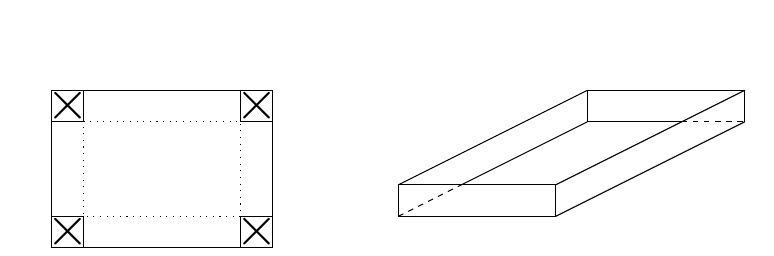
\begin{tikzpicture}[scale=0.4,every node/.style={scale=1}]
	\coordinate (A) at (0,0);
	\coordinate (B) at (7,5);
	\coordinate (C) at (1,1);
	\coordinate (D) at (6,4);
	\coordinate (E) at (7,0);
	\coordinate (F) at (0,5);
	\coordinate (G) at (6,1);
	\coordinate (H) at (1,4);
	\draw (A) rectangle (B);
	\draw (A) rectangle (C);
	\draw (B) rectangle (D);
	\draw (E) rectangle (G);
	\draw (F) rectangle (H);
	
	\path (A) -- (C) node[scale=2,midway]{$\times$};
	\path (B) -- (D) node[scale=2,midway]{$\times$};
	\path (E) -- (G) node[scale=2,midway]{$\times$};
	\path (F) -- (H) node[scale=2,midway]{$\times$};
	
	\draw [dotted] (H) -- (D) -- (G) -- (C) -- cycle;
	
%\draw (11,2)-- (14,2);
%\draw (14,2)-- (14,3);
%\draw (14,3)-- (11,3);
%\draw (11,3)-- (11,2);
%\draw (11,3)-- (15,5);
%\draw (15,5)-- (18,5);
%\draw (18,5)-- (18,4);
%\draw (18,4)-- (14,2);
%\draw (14,3)-- (18,5);
%\draw (15,4)-- (15,5);
%\draw [dash pattern=on 2pt off 2pt] (11,2)-- (13,3);
%\draw [dash pattern=on 2pt off 2pt] (16,4)-- (18,4);
%\draw (13,3)-- (15,4);
%\draw (15,4)-- (16,4);

\draw (11,1)-- (16,1);
\draw (16,1)-- (16,2);
\draw (16,2)-- (11,2);
\draw (11,2)-- (11,1);
\draw (11,2)-- (17,5);
\draw (17,5)-- (22,5);
\draw (22,5)-- (22,4);
\draw (22,4)-- (16,1);
\draw (16,2)-- (22,5);
\draw (17,4)-- (17,5);
\draw [dash pattern=on 2pt off 2pt] (11,1)-- (13,2);
\draw [dash pattern=on 2pt off 2pt] (20,4)-- (22,4);
\draw (13,2)-- (17,4);
\draw (17,4)-- (20,4);
\end{tikzpicture}
\end{center}
\newpage
\emptyhf
\begin{tikzpicture}[scale=1.3]%,xscale=1,every node/.style={scale=0.75}]
%\tkzSetUpPoint[shape=cross,size=20pt,color=teal,fill=teal]
\tkzInit[xmin=0,xmax=100,xstep=5, ymin=0,ymax=195,ystep=15]
\tkzGrid[sub,subxstep=1,subystep=5]
\tkzAxeXY
%\tkzFct[smooth,samples=100,domain = -7.5:8.75]{((\x)+6)*((\x)-6)/((\x)+8)}
%\tkzFct[samples=2,domain = -7.5:8.75]{-\x-6}
%\tkzDefPointByFct[draw,ref=A](-6)
%\tkzLabelPoint[above right](A){$A$}
%\tkzCrossPoint{A}
%\tkzDefPointByFct[draw,ref=B](-1)
%\tkzLabelPoint[above left](B){$B$}
%\tkzCrossPoint{B}
%\tkzText(8.5,2.5){$\mathcal{C}_{g}$}
%\tkzText(1.7,-2.7){$\mathcal{C}_{f}$}
\end{tikzpicture}

\newpage ~
\newpage
\pagestyle{savoirs}
\setcounter{exercice}{0}
\setcounter{probleme}{0}
\exercice % 1 
	\begin{enumerate}
		\item Résoudre graphiquement $h(t) > 2$.
		\item Déterminer graphiquement les antécédents de $2$ par $h$.
		\item Déterminer graphiquement $h(22)$.
		\item Déterminer graphiquement le maximum de la fonction $h$ et la valeur de $t$ pour laquelle on l'obtient.
		\item Déterminer graphiquement les valeurs de~$t$ pour lesquelles la fonction~$h$ est croissante et celles où la fonction~$h$ est décroissante.
		\item Exprimer les réponses de la question précédente sous forme d'intervalles de valeurs de $t$.
		\item Pour chacune des questions précédentes, exprimer en langage courant ce qui est demandé.
		\item Répondre maintenant aux questions de 1. à \addtocounter{enumi}{-2}\theenumi \addtocounter{enumi}{2}.
	\end{enumerate}
\exercice % 2
	\begin{enumerate}
		\item Résoudre $x - 2 = -2x + 1$.
		\item Tracer $f$ et $g$ dans un repère d'unité 1 cm. $x \in \left[-1~;~2\right], y \in \left[-3~;~3\right]$
		\item Que signifie $f(x) = g(x)$ ?
		\item Que signifie $f(x) \geqslant g(x)$ ?
	\end{enumerate}
\exercice % 3
\exercice % 4
\exercice % 5
\exerciceprime 
\exercice % 6
\exercice % 7
\exerciceprime

% Fin page 1

\exercice % 8
\exercice % 9
\exercice % 10

% Fin page 2

\exercice % 11
\exercice % 12
\exerciceprime

% Fin page 3

\exercice % 13
\exerciceprime
\exercice % 14

% Fin page 4

\exercice % 15

\probleme % 1
\probleme % 2


% Fin page 5

\end{document}


%
%%\exercicebareme{4}
%\exercicebareme{6}
%\exercicebareme{10}
%\exerciceunpoint
%\exercicebonus
%\FIN
%\BONNESVACANCES
%\BONCOURAGE
%\hrulefill